\documentclass{ximera}

%\ifdefined\HCode
%  \newcommand{\alttext}[1]{\HCode{<span class="sr-only">#1</span>}}
%\else
%  \newcommand{\alttext}[1]{} % Fallback for PDF view
%\fi


% MATH -----------------------------------------------------------
\newcommand{\nats}{\mathbb N}
\newcommand{\ints}{\mathbb Z}
\newcommand{\rats}{\mathbb Q}
\newcommand{\reals}{\mathbb R}
\newcommand{\complex}{\mathbb C}
\newcommand{\powerset}{\mathscr P}

%-------------------------------------------------------------

\pgfplotsset{compat=1.18}
\begin{document}
\begin{abstract}
 \end{abstract}

    \title{Exemplar Examples 25}
    
    \maketitle

    \begin{enumerate}

        
\item Let solve the integro-differential IVP \\$\displaystyle y^{\,\prime}(t)+\int_0^t (t-x) y(x)\,dx=3t$, $y(0)=0$.

\begin{enumerate}

\item First let's re-write the integral as a convolution $\displaystyle \left(f\ast g=\int_0^t f(x)g(t-x)\,dx\right)$.

\vfill


\item Now let's take the Laplace transform of both sides, and solve for $Y(s)=\mathcal{L}[y(t)]$.

\vfill
\vfill
\vfill

\item Now let's find the inverse Laplace transform of $Y(s)$.

\vfill
\vfill
\vfill



\end{enumerate}


\newpage


\item Let's consider the IVP $y'=-2x+\sqrt{x+\frac{1}{y^2}}$, $y(0)=1$.  Here is an (approximate) direction field for this differential equation on $[-1,2]\times [0,3]$.




\begin{figure}[h]
\centering
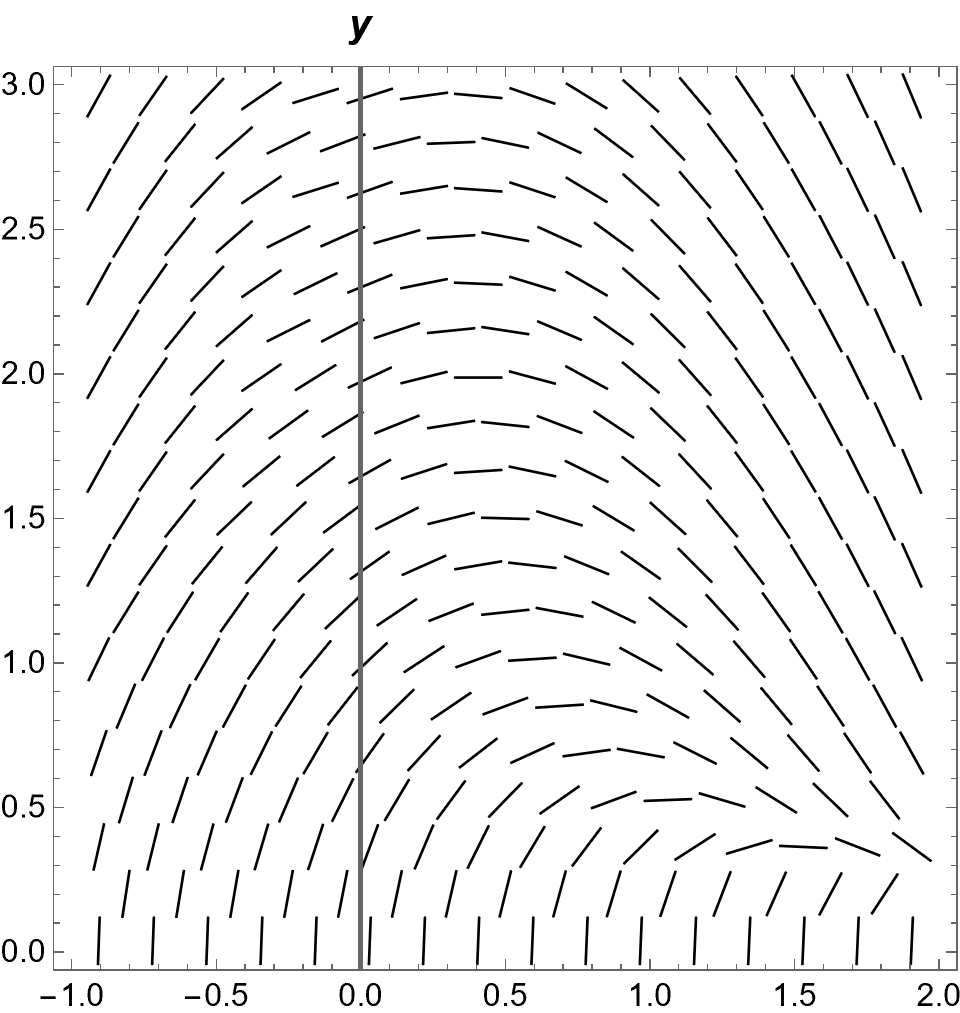
\includegraphics[scale=0.7,alt={A direction field.}]{ExemplarLastDirectionField.png}
   \caption{A direction field}
\end{figure}



\begin{enumerate}

\item Let's use Euler's method to approximate $y(1)$ using $5$ equal-sized steps.

\vfill

% y(0.2)\approx y_1=1+[-2*0+sqrt(0+1/1^2)]*(0.2)=1.2

% y(0.4)\approx y_2=1.2+[-2*0.2+sqrt(0.2+1/1.2^2)]*(0.2)\approx 1.30915014612

% y(0.6)\approx y_3=1.30915014612+[-2*0.4+sqrt(0.4+1/1.30915014612^2)]*(0.2)\approx 1.34749060376

% y(0.8)\approx y_3=1.34749060376+[-2*0.6+sqrt(0.6+1/1.34749060376^2)]*(0.2)\approx 1.3220359272

% y(1)\approx y_3=1.3220359272+[-2*0.8+sqrt(0.8+1/1.3220359272^2)]*(0.2)\approx 1.23631394323


% So about 1.24



\vfill

\item  Let's compare our estimate above with that which we can get by drawing.

\end{enumerate}

    \end{enumerate}



\end{document}
